In this section we will explain our methodology in more detail. At first we depict our subject, including the open-source projects we choose and the experimental environment we set up. Then we present each step of our approach.

\subsection{Subject systems}
We choose two open-source projects, \emph{Hadoop} and \emph{RxJava} as the subject systems of our case study. 
\emph{Hadoop}~\cite{hadoop2012:White} is a distributed system infrastructure developed by the Apache Foundation. \emph{Hadoop} performs data processing in a reliable, efficient, high fault tolerance, low cost and scalable manner. We choose \emph{Hadoop} since it is highly concerned with its performance and has been studied in prior research in mining performance data~\cite{markASE}. \emph{RxJava} is a library for composing asynchronous and event-based programs by using observable sequences and it carries the JMH benchmarks test options. \emph{RxJava} is a \emph{Java} VM implementation of reactive extensions. \emph{RxJava} provides a slew of performance micro-benchmarks, making it an appropriate subject for our study. The overview of the two studied systems is shown in Table~\ref{tab:subject}. 
 \begin{table}[tbh]
 	\centering
 	\small
	\caption{Overview of our subject systems.}
	\label{tab:subject}
	 	\begin{tabular}{llll}
 		\hline
 		Subjects&Version&Total lines of code (K)& No. of files \\\hline
 		Hadoop& 2.7.2              &1167      & 6,371     \\ 
 		Hadoop& 2.7.3			&1568		&6,439		\\\hline
 		RxJava&  2.0.0           & 164       & 1,107         \\ 
 		RxJava&  2.0.1			 &242		 &1,513		\\
 		RxJava&  2.0.2			&243			&1,524	\\
 		RxJava&  2.0.3			&244			&1,524	\\
 		RxJava&  2.0.4			&244			&1,526	\\\hline
 	\end{tabular}
\end{table}

\subsection{Predicting performance regression introducing changes}
In this subsection, we present our approach of predicting performance regression introducing changes. In general, we extract every commit and measures from the version control repositories (Git) of our subject systems and identify impacted test cases of each commit. Afterwards, we evaluate performance of each commit using either the related test cases or performance micro-benchmark. Then we perform statistical analysis on the performance evaluation results to identify performance regression. Finally, we build a prediction model based on the change measures to predict the JIT performance regression introducing changes.

\subsubsection{Filtering commits}
As the first step of our approach, we start off by filtering commits in order to focus on commits that are more likely to introduce performance regressions. In particular, we use \emph{git log} command to list all the files that are changed in each commit. We only extract the commits that have source code changes, i.e., changes to \emph{$.$java} files. 
\subsubsection{Extracting change measures}
To conduct our research, we extract the commit-level change measures from the CVS repositories of the projects and combined it with bug reports automatically. Simultaneously, we extract file-level change measures by manually, including EFC (having expensive function calls), CC (changing conditions), PEP (Passing expensive parameters), EL (having extra loops), EV (Using expensive variables) and IL (Introducing locks and synchronization). 
%The overview of the two studied systems is shown in Table~\ref{tab:subject}. 
\subsubsection{Identification of  performance regression introducing changes}
In more detail, we give a list of particular step:
\begin{enumerate}
\item \textbf{Identifying impacted tests.} In order to evaluate performance of each code commit, we use the tests and performance micro-benchmarks that are readily available in the source code of our subject systems. As mature software projects, each subject system consist of a large amount of test cases. 
%For example, \emph{Hadoop} release2.7.2 contains 1786 test cases in total. Exercising all test cases may cause two issues to our performance evaluation: 1) the test cases that are not impacted by the code change would dilute the performance impact from the code changes and introduce noise in the performance evaluation and 2) the large amounts of un-impacted test cases would requires extra resources for performance evaluation (e.g., much longer test running time). 

%Therefore, in this step, we leverage a heuristic to identify impacted tests for each commit. In particular, we find that \emph{Hadoop} test cases follow a naming convention that the name of the test files contain that same name of the source code files being tested. For example, a test file named \emph{TestFSNamesystem.java} tests the functionality of \emph{FSNamesystem.java}. Hence, for each changed source code file in a commit, we automatically identify the test files. 

%\noindent \textbf{Dealing with changed tests.} Some commits may change source code and test code at the same time. Such changed test cases would bias the performance evaluation if much testing logic is added, removed or modified in the test cases. In order to minimize the impact of changed test cases in performance evaluation, we opt to use the test code before the code change, since the new version of the test cases may include new features of the system, which is not the major concern of performance regression. However, in the cases where old test cases cannot compile or failed, we use the new test cases, since the failure of the compilation or the tests indicates that the old feature may be outdated. Finally, if both new and old test cases are failed or un-compliable, we do not include this test in the performance evaluation. In total, we have 132 tests with 106 commits that use the new tests to evaluate performance and 21 test with 19 commits that are not included in our performance evaluation. There exist only six commits that are not included at all because all of their tests are either un-compliable or failed.

%\noindent \textbf{Leveraging micro-benchmarks for \emph{RxJava}. }Fortunately, \emph{RxJava} provides a slew of micro-benchmarks with the goal of easing performance evaluation. We find that these performance micro-benchmarks are designed to evaluate performance of the software as a cross-cutting concern, instead of evaluating any particular features separately. Therefore, we opt to run all 76 micro-benchmarks from \emph{RxJava}. In the rest of this paper, we also refer these micro-benchmarks as test cases to ease the description of our results.

\item \textbf{Evaluating performance.}
In this step, we exercise the prepared test cases and the performance micro-benchmarks to evaluate performance of each commit. We setup our performance evaluation environment based on Azure node type Standard F8s (8 cores, 16 GB memory). In order to generate statistically rigorous performance results, we adopt the practice of repetitive measurements~\cite{peterfse} to evaluate performance. 
%In particular, each test or performance micro-benchmark are executed 30 times independently. We collect both domain level and physical level performance metrics during the tests. We measure the response time of each test case as domain level performance metric. A shorter response time indicating better performance of the software. We use a performance monitoring software named \emph{psutil}~\cite{psutil} to monitor physical level performance metrics, i.e., the CPU usage, Memory usage, I/O read and I/O write of the software, during the test.

\item \textbf{Statistical analyses on performance evaluation.}
%Statistical tests have been used in prior research and in practice to detect whether performance metric values from two tests reveal performance regressions \cite{AlGhmadi}. After having the performance evolution results, we perform statistical analyses to determine the existence and the magnitude of performance regression in a statistically rigorous manner. 
We use Student’s t-test to examine if there exists statistically significant difference (i.e., p-value $<$ 0.05) between the means of the performance metrics. A p-value $<$ 0.05 means that the difference is likely not by chance. 
%A t-test assumes that the population distribution is normally distributed. Our performance measures should be approximately normally distributed given the sample size is large enough according to the central limit theorem \cite{Chen:2014}.
T-test would only tells us if the differences of the mean between the performance metrics from two commits are statistically significant. On the other hand, effect sizes quantify such differences. 
\begin{comment}
Researchers have shown that reporting only the statistical significance may lead to erroneous results (i.e., if the sample size is very large, p-value can be small even if the difference is trivial). We use \emph{Cohen\textquotesingle s d} to quantify the effects~\cite{ES2006:Becker}. \emph{Cohen\textquotesingle s d} measures the effect size statistically and has been used in prior engineering studies~\cite{IST2007:Kampenes, ICSE2002:Kitchenham}. \emph{Cohen\textquotesingle s d} is defined as:
$$
Cohen\textquotesingle s \ d=\frac{mean(x1)-mean(x2)}{s}
$$
where \emph{mean(x1)} and \emph{mean(x2)} are the mean of two populations, and s is the pooled standard deviation~\cite{JohnWiley:2011}.
$$
\mathit{effect \ size} = \left\{ \begin{array}{ll}
trivial & \textrm{if $Cohen\textquotesingle s \ d  \leqslant 0.2$}\\
small & \textrm{if $0.2 < Cohen\textquotesingle s \ d \leqslant 0.5$}\\
medium& \textrm{if $0.5 < Cohen\textquotesingle s \ d \leqslant 0.8$}\\
large& \textrm{if $0.8 < Cohen\textquotesingle s \ d$}
\end{array} \right.
$$

\end{comment}
\end{enumerate}
\subsubsection{Data Preparation}
Before utilize the attributes to build our prediction models, we need to employ data cleaning to remove the data without file-level changes. We employ data reduction to make sure to remove highly correlated measures. And to avoid data skew, we apply data transformation to normalize data.
%属性相关性,归一化数据
\subsubsection{Build prediction model of JIT performance regression}
To predict the existence of performance regression introducing change, we will build the logistic regression model to firstlt to predict whether or not the change causes regression. If thus, we will build ordinal model to predict the magnitude of performance regression introducing change.

\begin{figure*}
	\centering
	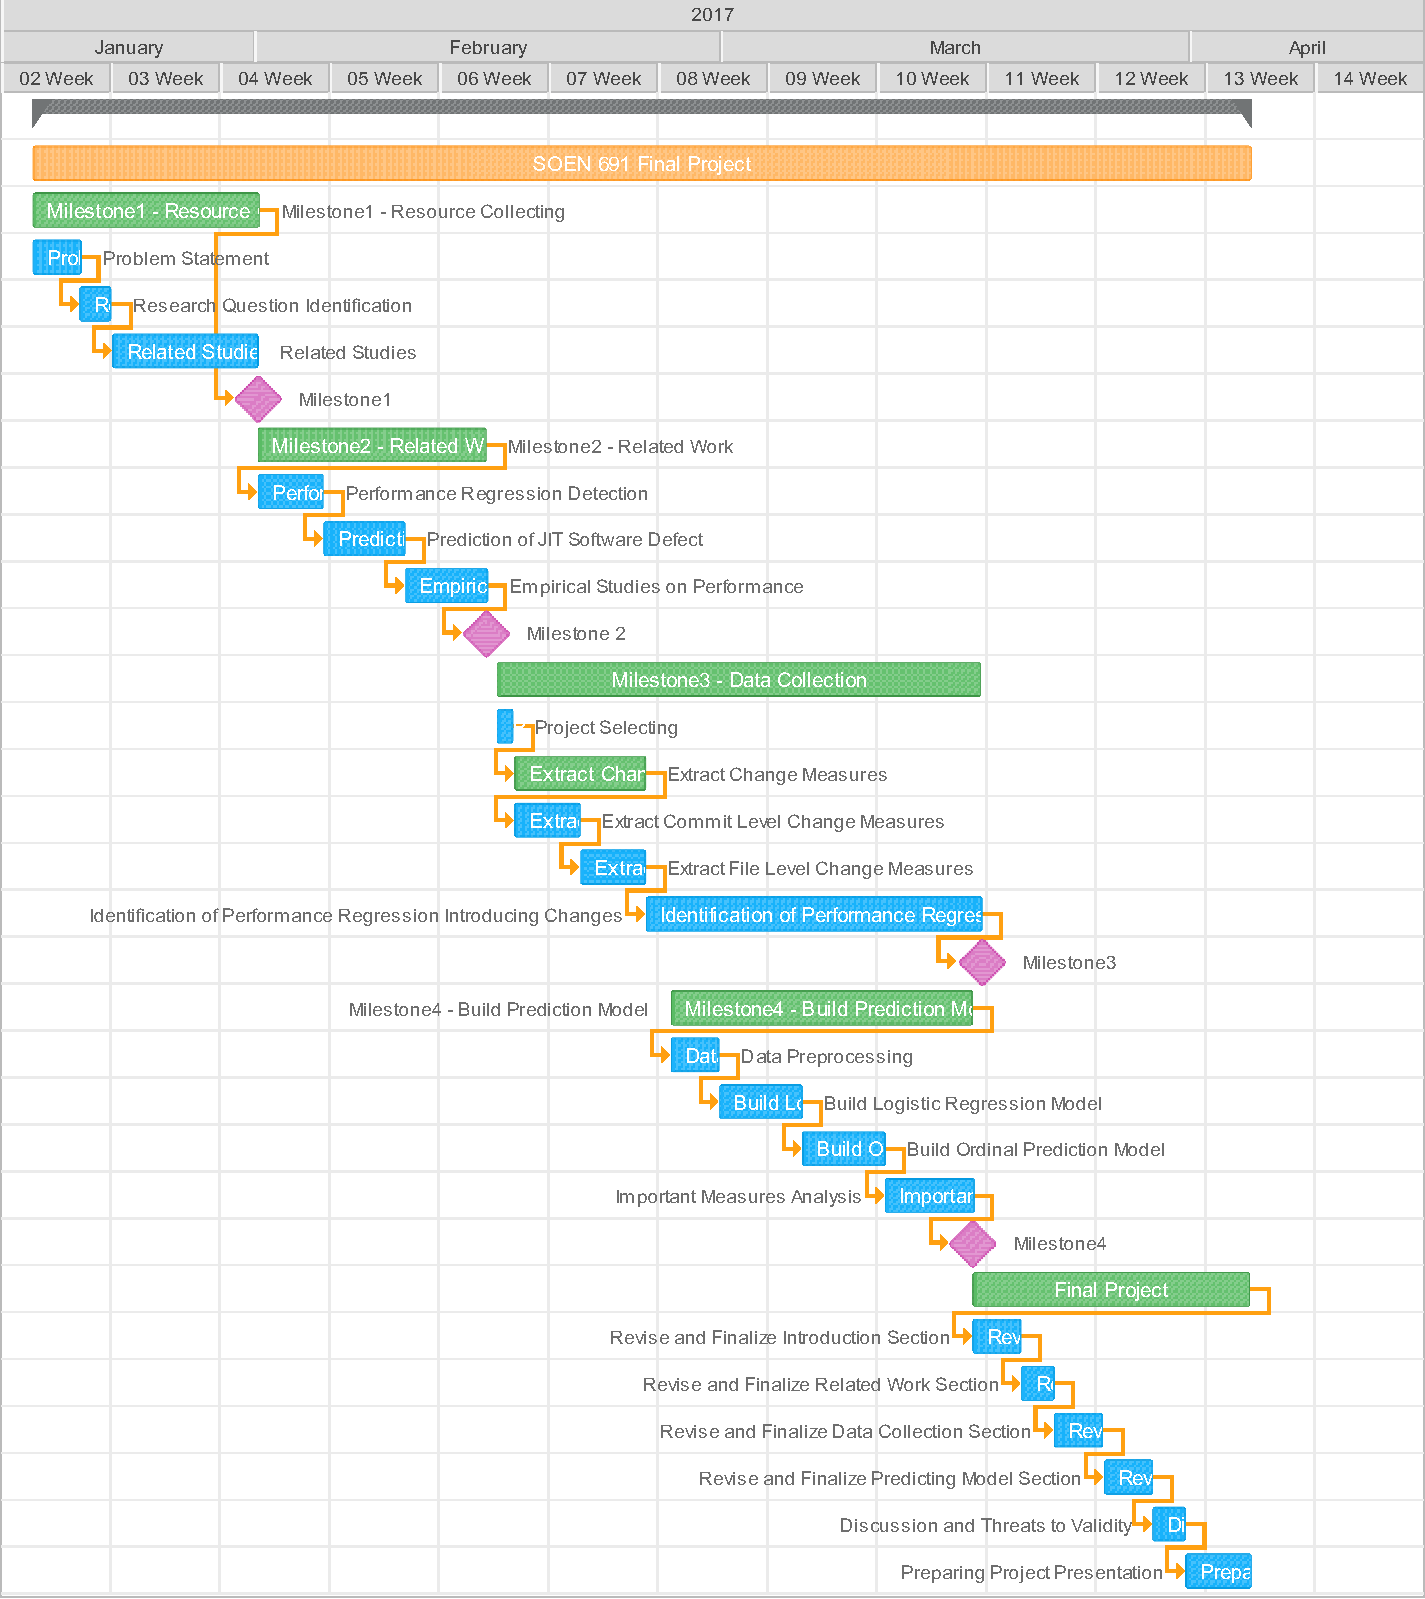
\includegraphics[width=\textwidth]{gantt_plot.pdf}
	\centering \caption{Gantt Chart of the project }
	{ (\url{https://app.ganttpro.com/shared/token/c645bd89d2023aae0eb33b33b628bdee70514115a86229ed7ec92c18455ca0f6})}
	\label{fig:gantt}
\end{figure*}
